

\newcommand{\ysc}[0]{0.3}
\newcommand{\xsc}[0]{0.3}


\begin{tikzpicture}[yscale =\ysc, xscale=\xsc, radius=1.5cm]


\begin{scope}[xshift = 0cm]
\draw[-](0,0) -- (8,0);

\foreach \x in {0,1,2,...,8}{
\begin{scope}[xshift=\x cm]
\draw[-](0, 0) -- (0, 2);
\draw[-, fill](0, 0) -- (0.1, 0.2) -- (-0.1, 0.2) --(0,0);
\end{scope}
}
\draw[-](0, 2) -- (8, 2);


\draw[<-, color=black](-0.6, 0) -- (-2,0)node[left]{};
\draw[->, color=black](-0.8, 0.7) -- (-0.8, -0.7)node[below]{};
\draw[<-, color=black](-0.9,-1.06) arc[start angle=225, end angle=135];
\node at (-1.7, 0.4){};

\draw[->, color=black](8.6, 0) -- (10,0)node[right]{};
\draw[->, color=black](8.8, 0.7) -- (8.8, -0.7)node[below]{};
\draw[<-, color=black](8.9,1.06) arc[start angle=45, end angle=-45];
\node at (9.7, -0.4){};
\node at (4, -2)[below]{$p(x)= p$};
\end{scope}


\begin{scope}[xshift = 17cm]
\draw[-](0,0) -- (8,0);



\foreach \x in {1,2,...,8}{
\begin{scope}[xshift=\x cm]
\draw[-](0, 0) -- (0, \x*0.25);
\draw[-, fill](0, 0) -- (0.1, 0.2) -- (-0.1, 0.2) --(0,0);
\end{scope}
}

\draw[-](0, 0) -- (8, 2);


\draw[<-, color=black](-0.6, 0) -- (-2,0)node[left]{};
\draw[->, color=black](-0.8, 0.7) -- (-0.8, -0.7)node[below]{};
\draw[<-, color=black](-0.9,-1.06) arc[start angle=225, end angle=135];
\node at (-1.7, 0.4){};

\draw[->, color=black](8.6, 0) -- (10,0)node[right]{};
\draw[->, color=black](8.8, 0.7) -- (8.8, -0.7)node[below]{};
\draw[<-, color=black](8.9,1.06) arc[start angle=45, end angle=-45];
\node at (9.7, -0.4){};
\node at (4, -2)[below]{$p(x)= p \cdot \dfrac{x}{l}$};
\end{scope}

\begin{scope}[xshift = 34cm]
\draw[-](0,0) -- (8,0);

\foreach \x in {0,1,2,...,7}{
\begin{scope}[xshift=\x cm]
\draw[-](0, 0) -- (0, 2-\x*0.25);
\draw[-, fill](0, 0) -- (0.1, 0.2) -- (-0.1, 0.2) --(0,0);
\end{scope}
}
\draw[-](0, 2) -- (8, 0);


\draw[<-, color=black](-0.6, 0) -- (-2,0)node[left]{};
\draw[->, color=black](-0.8, 0.7) -- (-0.8, -0.7)node[below]{};
\draw[<-, color=black](-0.9,-1.06) arc[start angle=225, end angle=135];
\node at (-1.7, 0.4){};

\draw[->, color=black](8.6, 0) -- (10,0)node[right]{};
\draw[->, color=black](8.8, 0.7) -- (8.8, -0.7)node[below]{};
\draw[<-, color=black](8.9,1.06) arc[start angle=45, end angle=-45];
\node at (9.7, -0.4){};
\node at (4, -2)[below]{$p(x)= p \cdot \left(1-\dfrac{x}{l}\right)$};
\end{scope}



\end{tikzpicture}
